\section{Internal Forces}

Internal forces of a member can be determined by creating an imaginary cut in a member, and then solving for the internal shear force, normal force, and bending moment (which, after the cut, become "external" forces that can be solved for). 

To determine how the internal shear force and bending moment change throughout the member, shear force and bending moment diagrams are created. Shear force diagrams provide a graphical representation of the internal shear force within a member, and bending moment diagrams provide a graphical representation of the internal bending moment within a member. 

\begin{figure*}[!h]
\centering
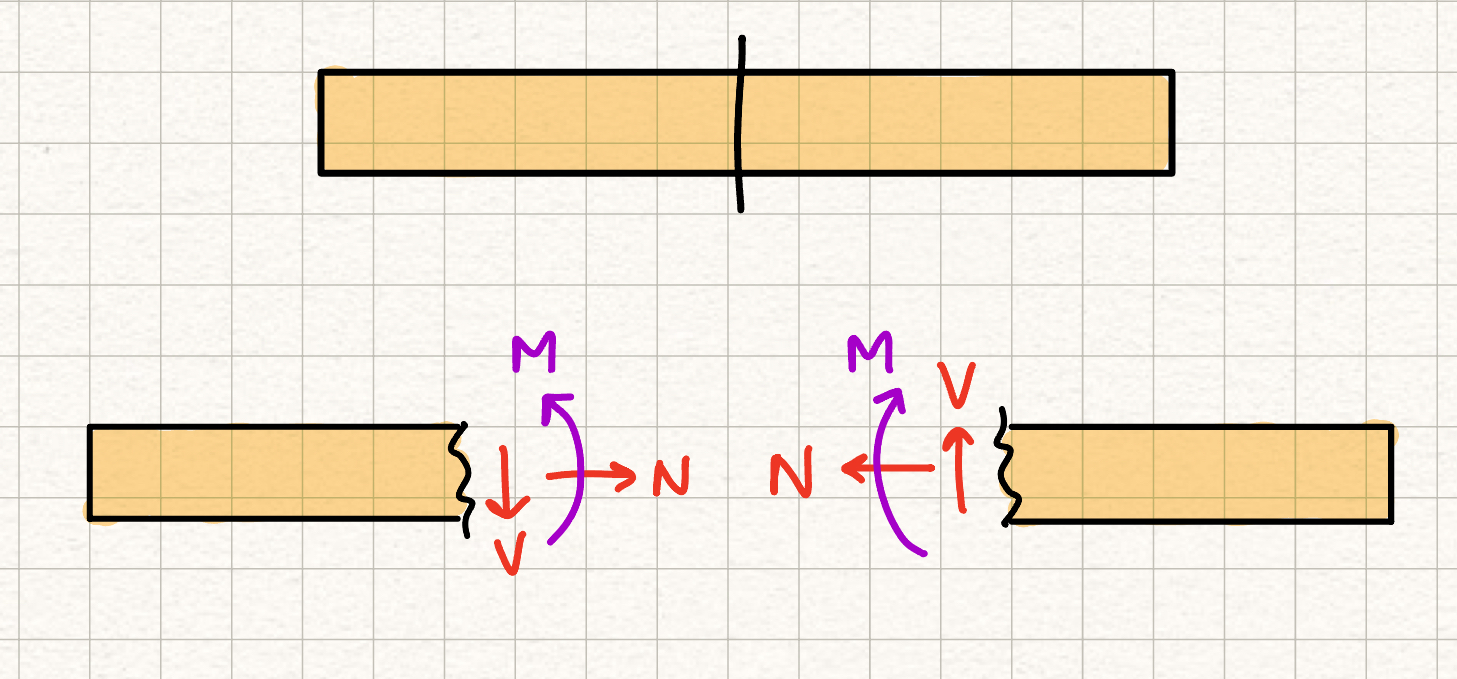
\includegraphics[angle=0, width=5 in]{IntForceFigures/IntForces.jpg}
\vspace{-2mm}
\caption{\small Internal shear force (V), internal normal force (N), and internal moment (M).}
\vspace{-3mm}
\label{Fig:IntForces}
\end{figure*}

%starts in lecture 19

\subsection{Sign Conventions}

\begin{figure*}[!h]
\centering
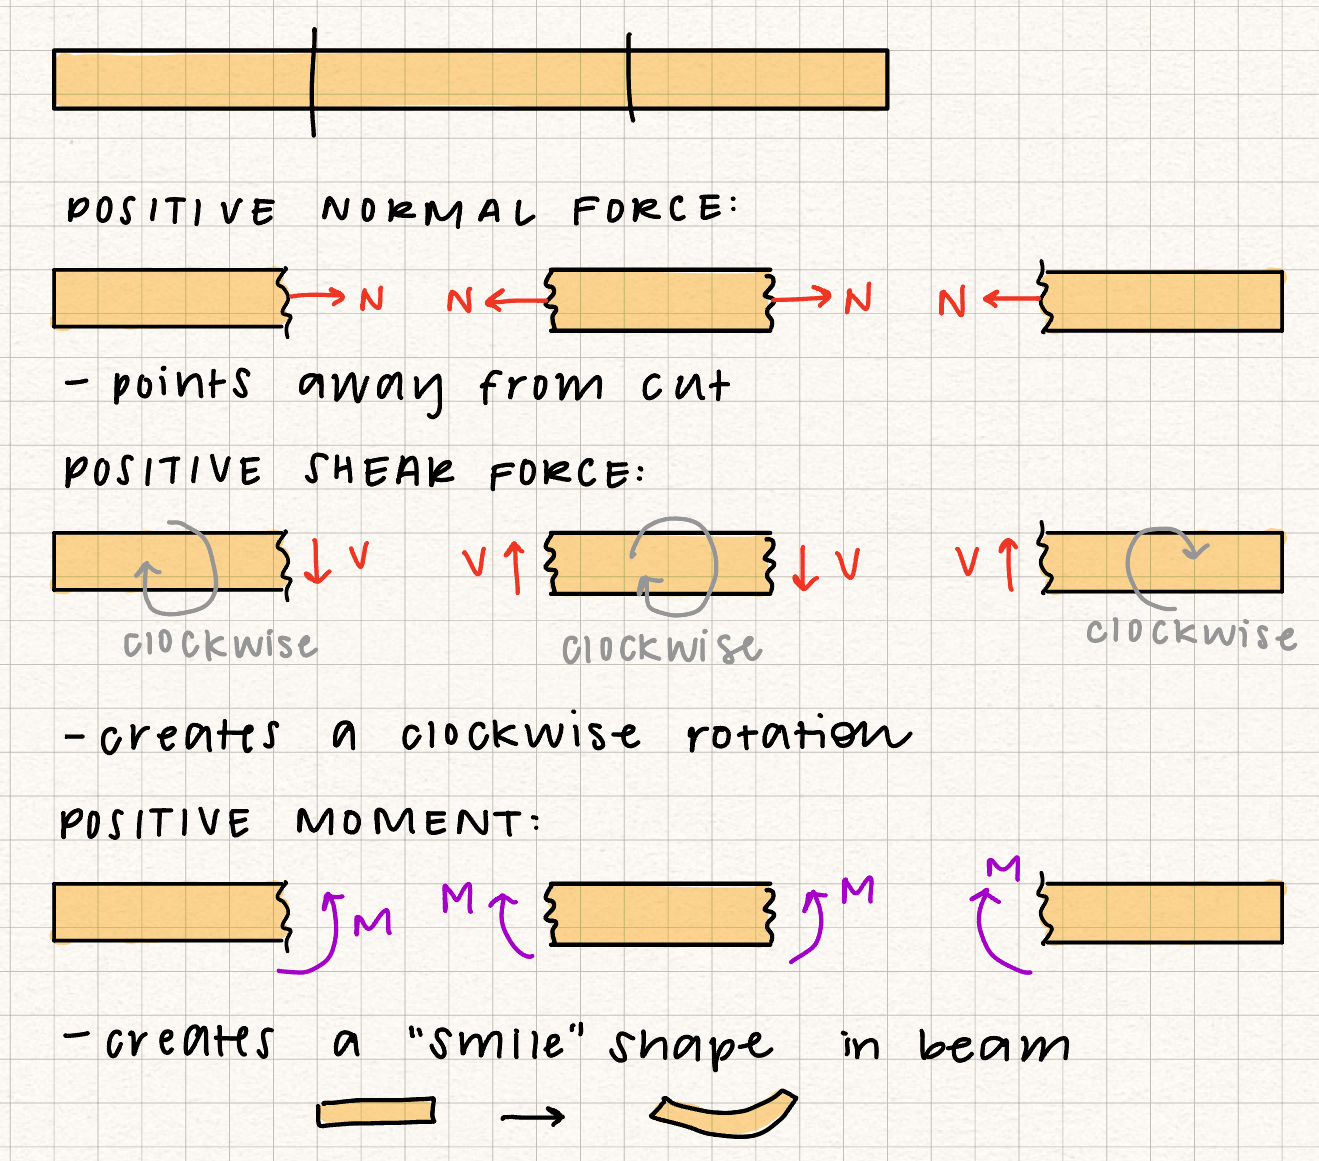
\includegraphics[angle=0, width=\textwidth]{IntForceFigures/SignConventions.jpg}
\vspace{-2mm}
\caption{\small Sign conventions for internal forces and moments}
\vspace{-3mm}
\label{Fig:SignConventions}
\end{figure*}


\subsection{General Procedure}

Creating a shear force and bending moment diagram allows us to create a graphical representation of $V$ and $M$ as a function of the position along the beam, $x$. Therefore when creating internal loading diagrams we are trying to write equations for $V(x)$ and $M(x)$.

\begin{figure*}[!h]
\centering
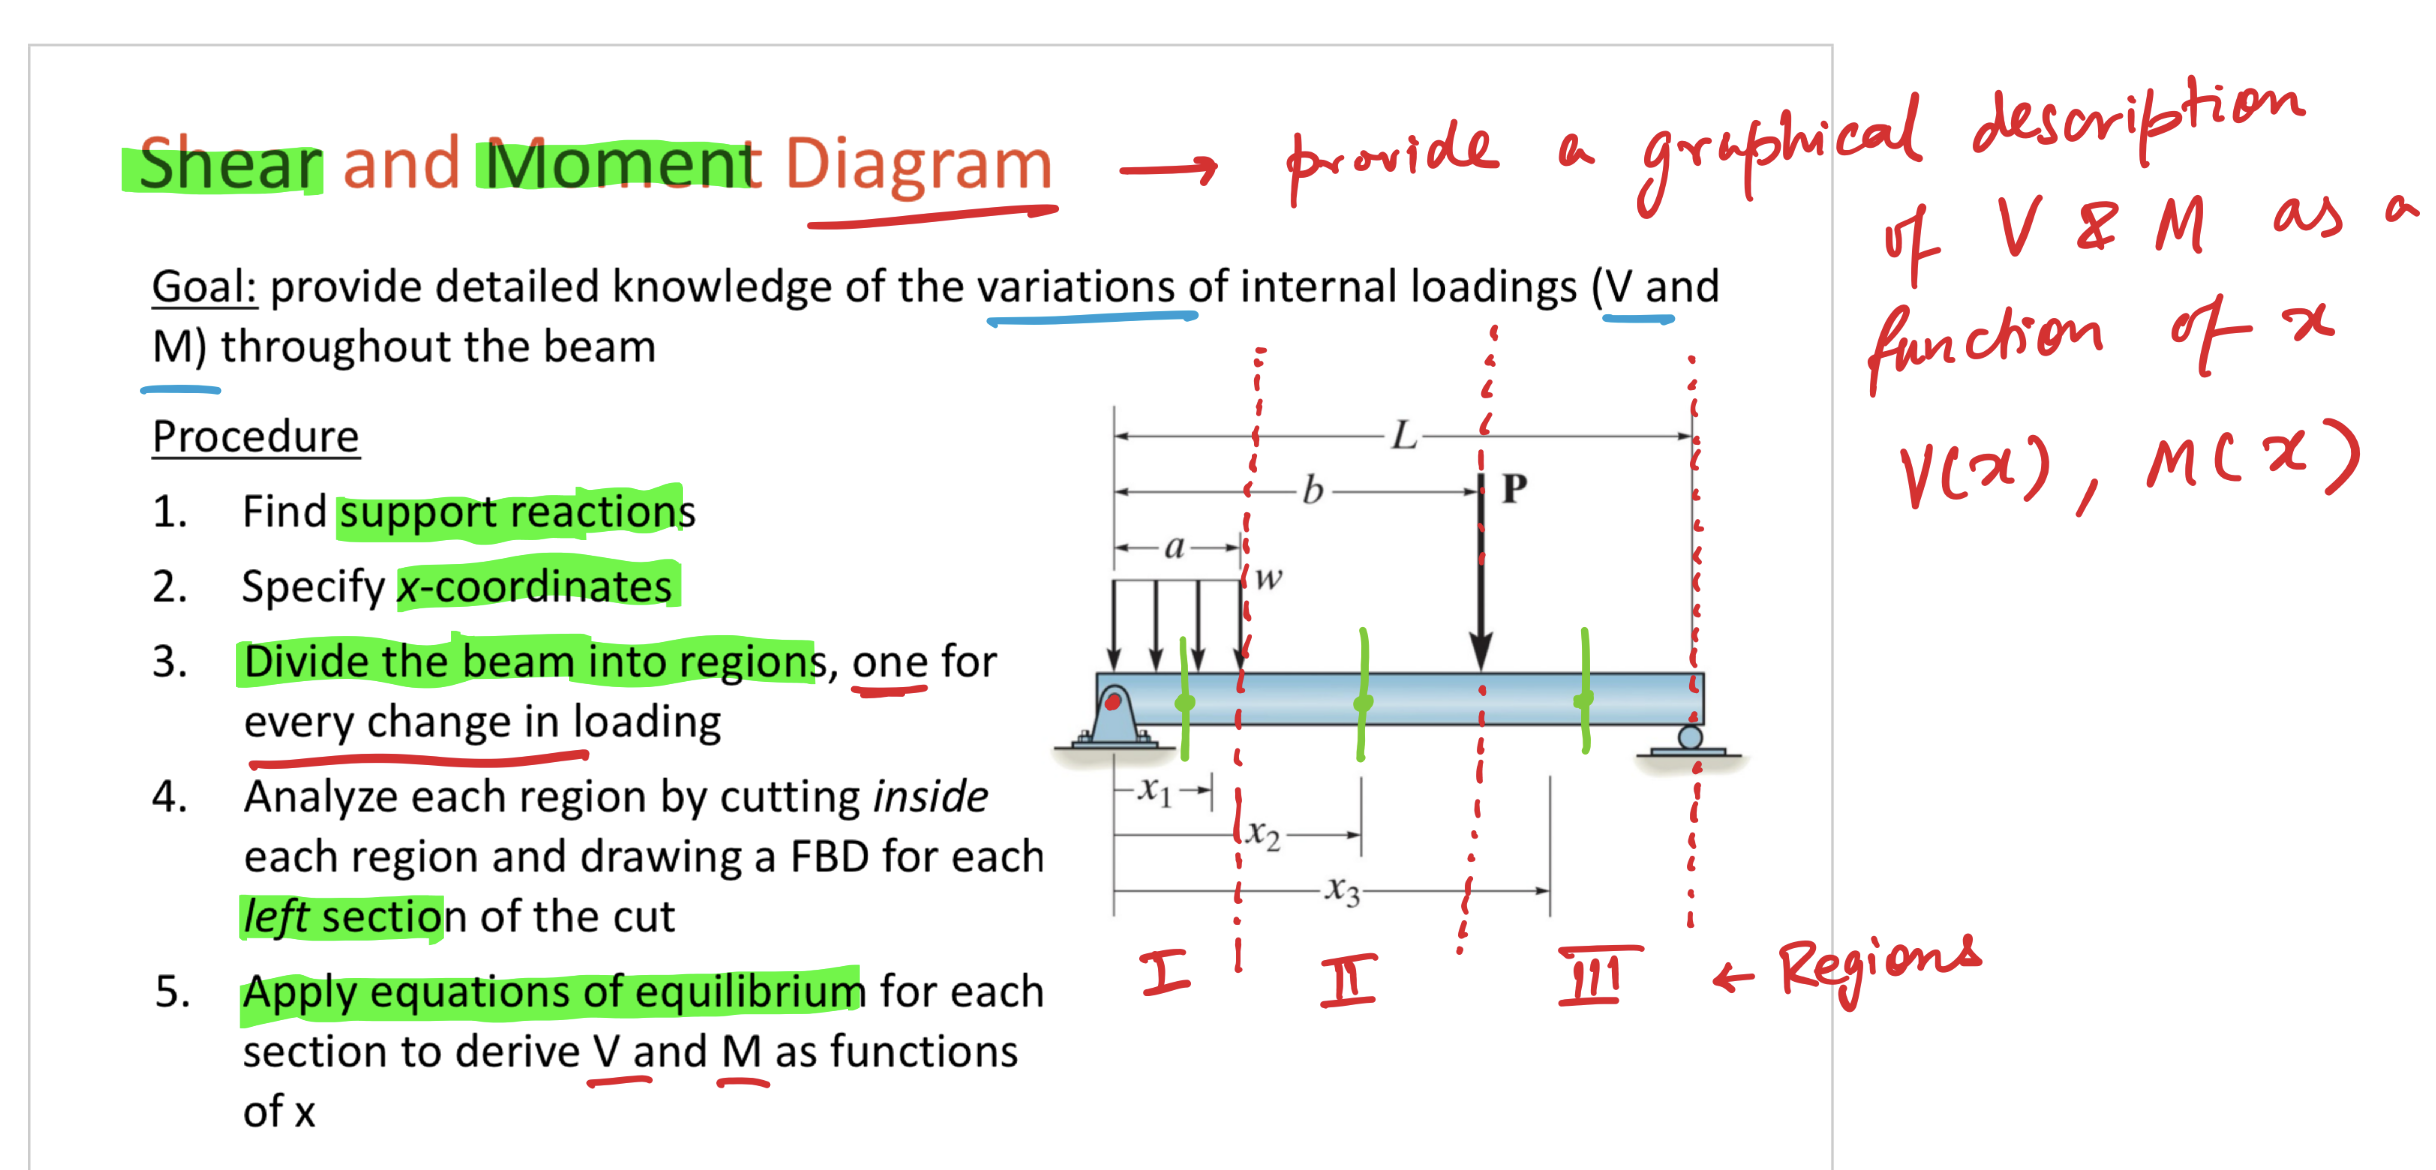
\includegraphics[angle=0, width=\textwidth]{IntForceFigures/DiagramProcedure.png}
\vspace{-2mm}
\caption{\small \blue{Taken from TAM 210 Lecture 22}}
\vspace{-3mm}
\label{Fig:DiagramProcedure}
\end{figure*}

\begin{figure*}[!h]
\centering
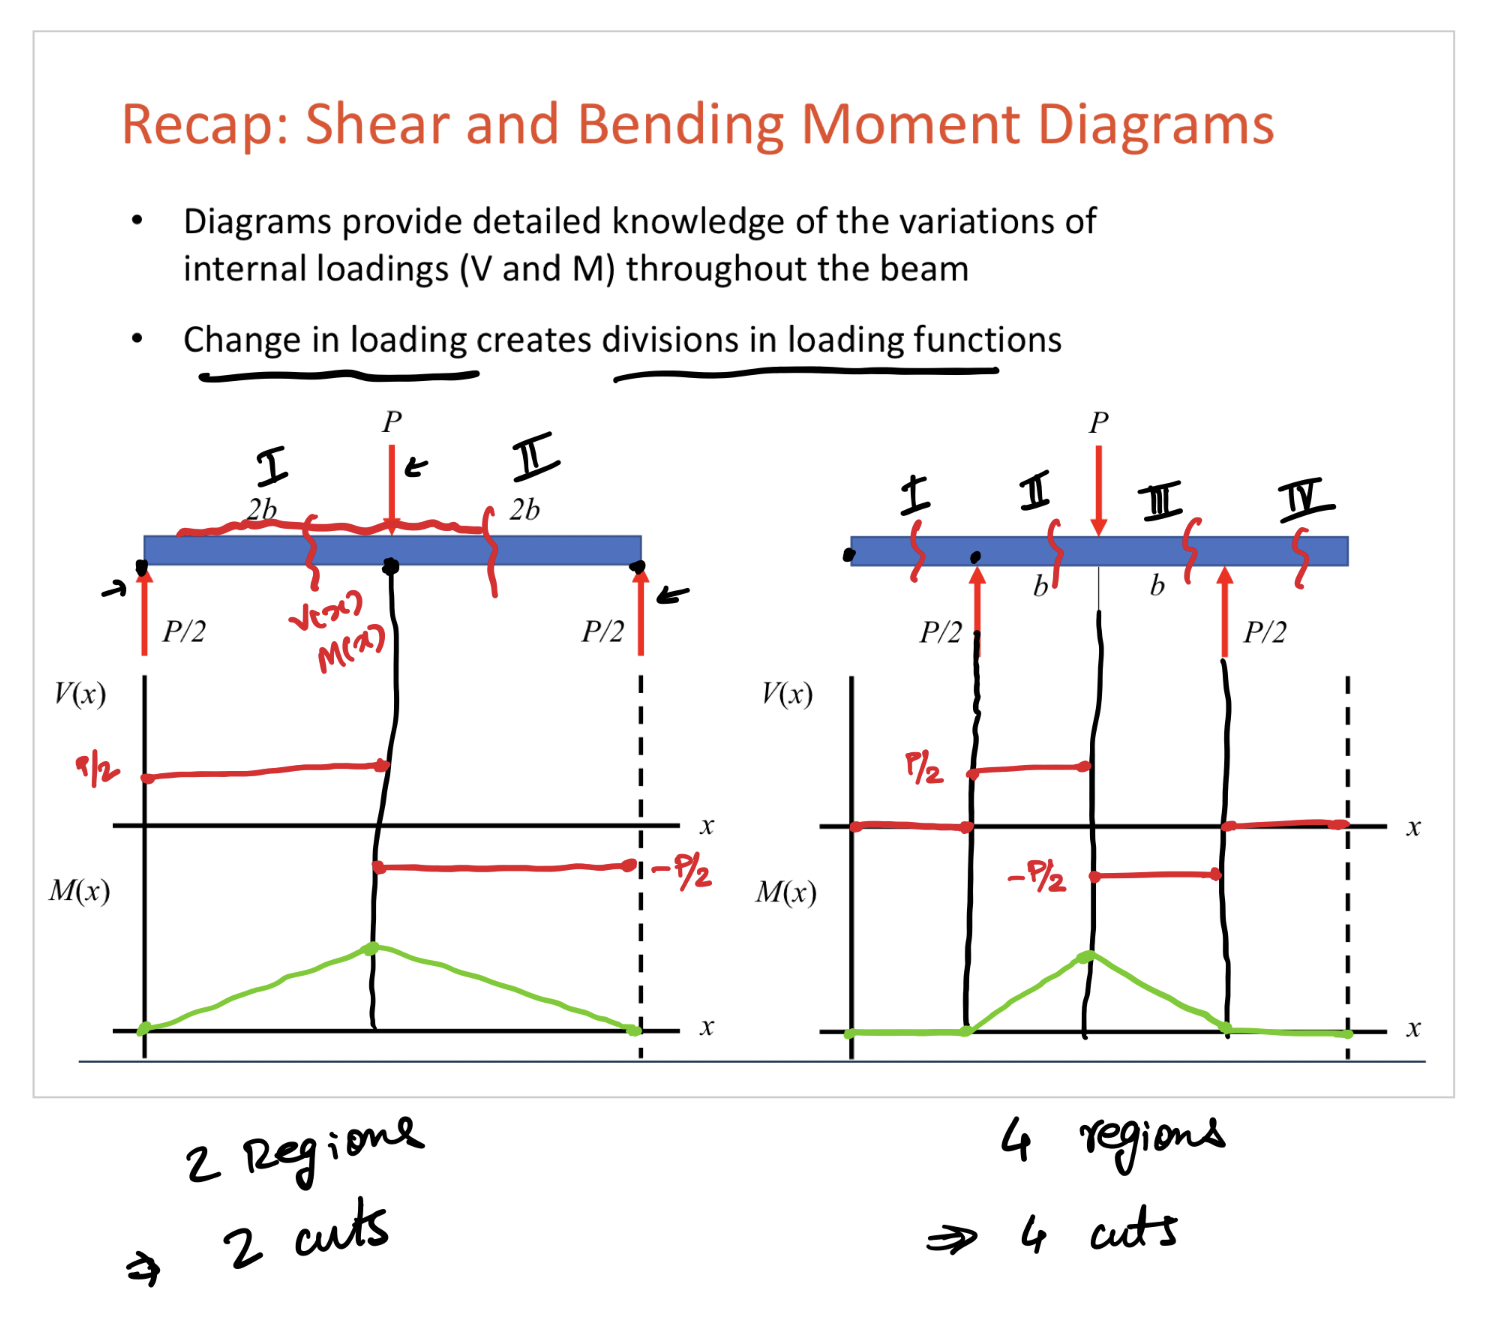
\includegraphics[angle=0, width=\textwidth]{IntForceFigures/IntLoadRecap.png}
\vspace{-2mm}
\caption{\small \blue{Taken from TAM 210 Lecture 23}}
\vspace{-3mm}
\label{Fig:DiagramProcedure}
\end{figure*}

\subsection{\red{General Rules}}

\begin{enumerate}
    \item When there is an external concentrated force or moment, there will be a "jump" in the shear force or bending moment diagram
    \item $w(x)$, $V$, and $M$ are related via the following relationship: 
\end{enumerate}

\begin{figure*}[!h]
\centering
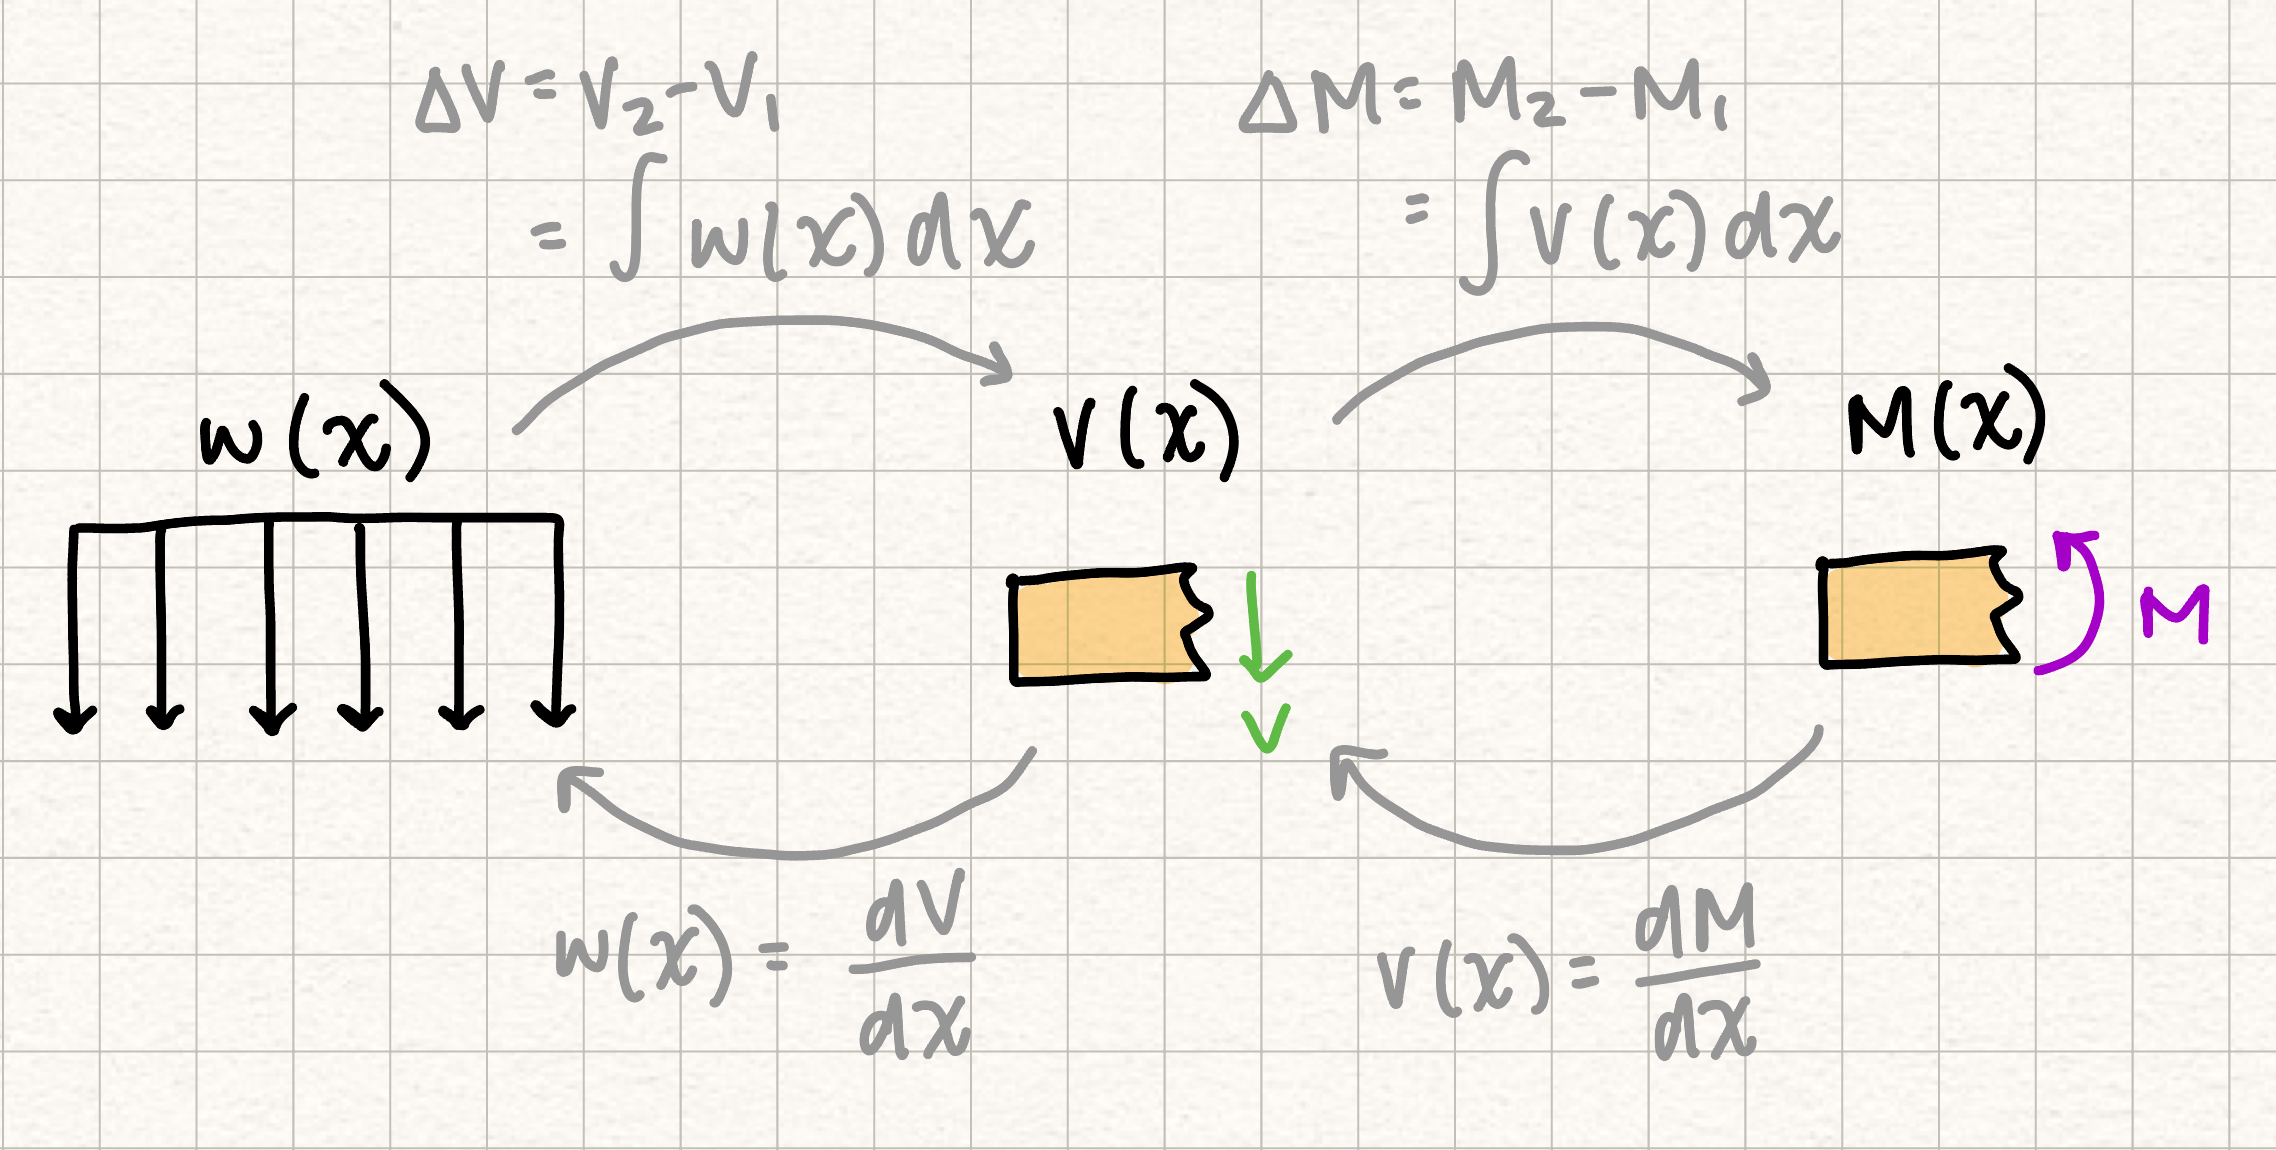
\includegraphics[angle=0, width=\textwidth]{IntForceFigures/IntDerivRelationships.jpg}
\vspace{-2mm}
\caption{\small \blue{See TAM 210 Lecture 25}}
\vspace{-3mm}
\label{Fig:IntForceRelationships}
\end{figure*}

\subsection{\red{Shear Force Diagram}}

%Lecture 22, 23, 24

\subsection{\red{Bending Moment Diagram}}

%Lecture 22, 23, 24
